\chapter{绪论}
\section{研究课题的背景与意义}
在自然界,外骨骼是一种能为生物内部柔软组织和器官提供保护的外部结构,如虾、蟹、昆虫等节肢动物体表坚韧的几丁质的骨骼。近些年的科幻电影中,频繁出现一些能够提高人体机能的可穿戴外骨骼,如《钢铁侠》中的Mark战甲、《流浪地球》中火石救援队的作战装甲等。

\begin{figure}[htb]
    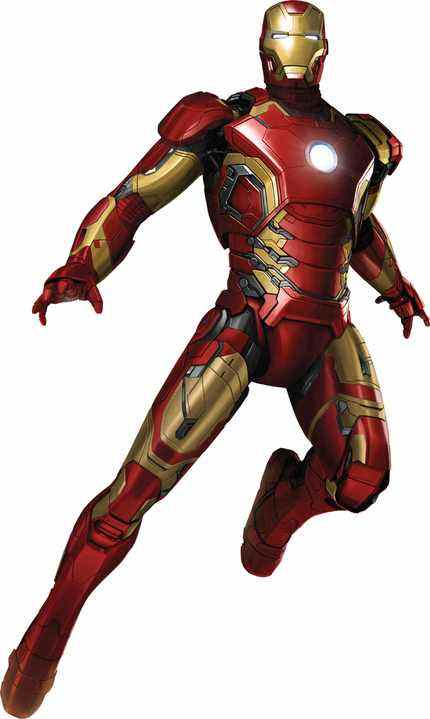
\includegraphics[width=6cm]{fig/p2_mark.jpg}
    \caption{电影钢铁侠中的Mark战甲}
    \label{fig:mark}
\end{figure}

实际上,外骨骼机器人技术作为一个富有活力的课题,在人体运动机能提升\cite{p1}和医疗康复\cite{p2}领域的研究已存在超过半个世纪。外骨骼机器人是一种综合了传感器技术、信号处理、智能控制、人机交互的一体化可机械装置。随着机器人技术的发展,传统的独立作业机器人,如工业机器人、无人机等,已相对成熟,而具有人机协作功能的机器人成为研究热点。外骨骼机器人作为其最典型的应用,正逐渐受到研究人员的重视。近些年随着检测技术、控制理论、人工智能等相关领域的发展,可穿戴设备的研究取得了巨大的进步(XXX)。

在现代战争,士兵需要背负越来越多的武器和设备,进行远距离机动和长时间作战,其体力和耐力受到严重考验。使用助力外骨骼可以有效减轻士兵负担,从而提高单兵作战能力,提高其战场生存能力。另一方面,随着人口老龄化趋势的增加,和人们健康意识的提高,医疗康复设备的需求量日益增长。根据第二次全国残疾人抽样调查和第六次人口普查的数据推算,2013年中国的肢体残疾者数量达到了3700万,占全国人口的2.65\% \cite{p3},下肢外骨骼机器人使广大残疾人和老年人获得了重新行走的可能。

下肢外骨骼的研究主要聚焦于三个方向:一是为正常人设计、旨在提高人体运动机能的助力设备,其主要应用于军事作战、抢险救灾和工业负重;二是为运动障碍者设计的助力设备,穿戴者可以在外骨骼的辅助下重新获得行走能力;三是可穿戴式康复医疗设备,旨在通过预先设定的重复性动作帮助患者恢复身体机能。本项目研究为正常人设计的脚踝式助力外骨骼,在运动过程中为穿戴者提供关节力矩辅助,从而减轻穿戴者的运动负担、提高穿戴者的运动机能。
